\documentclass{if-beamer}

% --------------------------------------------------- %
%                  Presentation info	              %
% --------------------------------------------------- %
\title[Lecture 1]{Lecture 1}
\subtitle{Syllabus Overview and Getting to Know You}
\author{Instructor: Ashley Gannon}
\date{ISC3313 Fall 2021}
\logo{
\includegraphics[scale=0.08]{FSULogo.png}
}
\subject{Presentation subject} % metadata

%\graphicspath{{figures/}}
% --------------------------------------------------- %
%                    Title + Schedule                 %
% --------------------------------------------------- %

\begin{document}

\begin{frame}
  \titlepage
\end{frame}

\section{Syllabus overview}

\begin{frame}
\frametitle{Course overview}
{\textbf{Course content:}} \\
{This course introduces you to the science of computations. Algorithms
	for standard problems in computational science are presented. The
	basics of the object-oriented programming language C++ are taught to
	facilitate the implementation of algorithms.} \\[0.2cm]
{\textbf{Course objectives:}} \\
\begin{itemize}
	\item Identify the components of scientific computing
	\item Identify standard problems in scientific computing
	\item Implement basic algorithms for standard problems in computational science using \texttt{C++}.
	\item Write, debug, and verify computer programs
	\item Output results of computer simulations in a meaningful manner
\end{itemize}
\end{frame}


\begin{frame}
\textbf{Grading Policy:} \\[0.1cm]
The grading for this course will be based upon participation, weekly homework assignments, and a final project. The weights are given as follows:
\begin{itemize}
	\item Participation (10\%)
	\item Homework (50\%)
	\item Capstone Project (40\%)
\end{itemize}
\vspace{.25cm}
\textbf{Late Homework Policy:}\\
Late homework will be treated as follows: the maximum achievable grade on a homework assignment will decrease by 10 points for every business day late. After 5 business days or more, the maximum penalty is capped at 50 points. In other words, a student is encouraged to submit any late homework \textbf{by December 3rd, 2020} for up to 50 percent credit. Homework submitted after will not be graded.
\end{frame}

\begin{frame}
\textbf{Capstone Project:} \\[0.1cm]
This course requires a final “capstone project” in order to fulfill FSU’s
Computer Competency Requirement. Completion of the
project requires a working program demonstrating knowledge of the subject matter taught in the course and a written report (3-5 pages).\\
\vspace{.25cm}
Grading of the program submitted is based on the student's ability to explain the problem and solution, correctness, efficiency, and clarity. In other words, the program must compile and run, must be a correct implementation of a procedure to solve the problem, and must report information about the solution to the problem that can be presented in a table or a plot. The grade percentages for the Capstone project are as follows:
\begin{itemize}
	\item \texttt{C++} program (60\%)
	\item written report (30\%)
	\item oral presentation(10\%)
\end{itemize}

\end{frame}

\section{Introductions}
\begin{frame}
	\frametitle{Introductions + BINGO Activity}
	Let's take some time to get to know each other. \\\vspace{0.25cm}
	\href{https://docs.google.com/presentation/d/1RA8mvQN5wGJxhHejI15yhpj0bJaxpHsFAa3dCMYQcvM/edit?usp=sharing}{Personal slides}
	
\end{frame}



\section{What is scientific computing?}
\begin{frame}
\frametitle{An interdisciplinary field}
\begin{figure}
	\center
	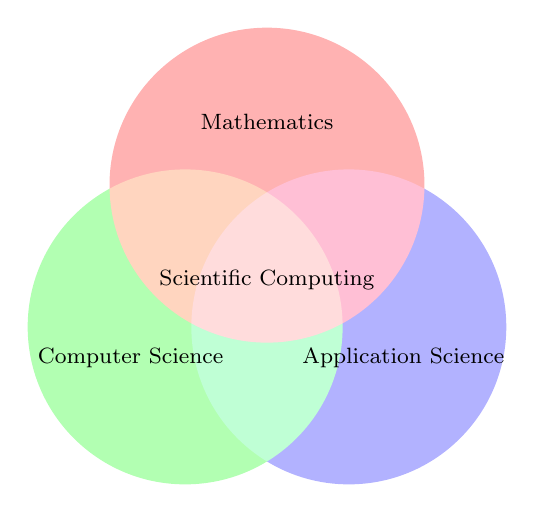
\begin{tikzpicture}
	\begin{scope}[blend group = soft light]
	\fill[red!30!white]   ( 90:1.2) circle (2);
	\fill[green!30!white] (210:1.2) circle (2);
	\fill[blue!30!white]  (330:1.2) circle (2);
	\end{scope}
	\node at ( 90:2)    {\footnotesize Mathematics};
	\node at ( 210:2)   {\footnotesize Computer Science};
	\node at ( 330:2)   {\footnotesize Application Science};
	\node [font=\small] {\footnotesize Scientific Computing};
	\end{tikzpicture}
\end{figure}
\end{frame}

\begin{frame}
\frametitle{Problems in Scientific Computing}
A problem in the field of scientific computing (computational science) typically requires: \\[0.2cm]
\begin{itemize}
	\item understanding of physical principles
	\item the development or use of a mathematical model
	\item the development or implementation of numerical algorithms
	\item large-scale (parallel) computations
	\item verification of the code for the problem at hand
\end{itemize}
\end{frame}

\begin{frame}
\frametitle{The third pillar of science}
Computations have provided a new ability to probe the natural world.
\begin{figure}
	\center
	\includegraphics[width=0.6\textwidth]{threepillars.png}
\end{figure}
\end{frame}

\section{Overview of computational science topics}

\begin{frame}
\frametitle{Fundamental numerical math topics}
Solutions to these types of problems are essential in computational science:
\begin{itemize}
	\item linear algebra (solving systems of equations): $Ax=b$
	\item solving nonlinear equations: find $x$ such that $x = \sin({x})$
	\item interpolation and fitting of data: $y = mx + b$
	\item approximate integrals: $\int_{a}^{b} f(x) dx$
	\item solving differential equations: $\frac{dy}{dt} =
	\exp{(-\lambda t)}, \quad y(0) = y_{0}$
\end{itemize}
\end{frame}

\begin{frame}
\frametitle{Fundamental computer science topics}
The following computer science topics are also important: \\
\begin{itemize}
	\item object-oriented programming (and debugging!)
	\item data structures
	\item parallel computing
\end{itemize}
\end{frame}

\begin{frame}
\frametitle{Scientific applications}
There are many scientific applications to explore: \\
\begin{itemize}
\item Engineering (solid mechanics, materials science, fluid
dynamics, vibration dynamics, ...)
\item Biology (computational neuroscience, vesicles, population dynamics, computational genetics,...)
\item Machine learning (autonomous navigation, ...)
\item Data science (fraud and risk detection, healthcare, internet
search, advanced image recognition, ...)
\end{itemize}
In fact there are too many to list!
\end{frame}

\section{Why be a computational scientist?}

\begin{frame}
\frametitle{Why be a computational scientist?}
Money!
\begin{figure}
	\center
	\includegraphics[width=0.35\textwidth]{money.jpg}
\end{figure}
According to Glassdoor.com:
\begin{figure}
	\center
	\includegraphics[width=0.6\textwidth]{glassdoor.png}
\end{figure}
\end{frame}

% --------------------------------------------------- %
%                      Presentation                   %
% --------------------------------------------------- %

\end{document}
